\begin{frame}
    \begin{exampleblock}{Exercise I}
        \begin{enumerate}
            \item Get the Arduino\textregistered{} \acs{ide} of your choice.
            \item Connect the board to your \acs{pc}.
            \item Install the \ac{bsp} for your board.
            \item Run the example project ``Blink''.
            \item Extend the example project to log \texttt{On} or \texttt{Off} when toggling the \acs{led}.
        \end{enumerate}
        \par Hint:
        \begin{itemize}
            \item \href{https://www.arduino.cc/reference/en/language/functions/communication/serial/begin/}{\mintinline{c}{Serial.begin()}}
            \item \href{https://www.arduino.cc/reference/en/language/functions/communication/serial/println/}{\mintinline{c}{Serial.println()}}
        \end{itemize}
    \end{exampleblock}
\end{frame}

\begin{frame}{Solution: Exercise I}
    \begin{listing}[H]
        \inputsource[fontsize=\fontsize{8}{8}]{c}{arduino/blink-logging.c}
        \caption{Solution for Exercise I.}
        \label{lst:arduino:exercise:1:solution}
    \end{listing}
\end{frame}

\begin{frame}{Solution: Exercise I}
    \begin{figure}
        \begin{tikzpicture}
            \draw (2,4) node[rp2040] (rp20401) {};
        \end{tikzpicture}
        \caption{Circuit for Exercise I}
    \end{figure}
\end{frame}

\begin{frame}{Solution: Exercise I}
    \begin{figure}
        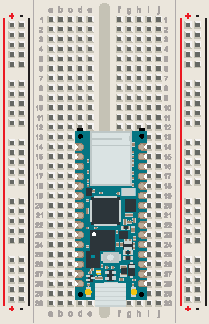
\includegraphics[width=0.35\textwidth]{images/microcontroller/exercises/exercise-1-solution.pdf}
        \caption{Solution for Exercise I.}
    \end{figure}
\end{frame}
